\documentclass[crop,tikz]{standalone} 
\usepackage{tikz, amsmath, amssymb, graphicx} 

\usetikzlibrary{positioning, shapes.geometric} 

\begin{document} 

\begin{tikzpicture}


\node[inner sep=0pt] (sim:0.05) at (0,0) {
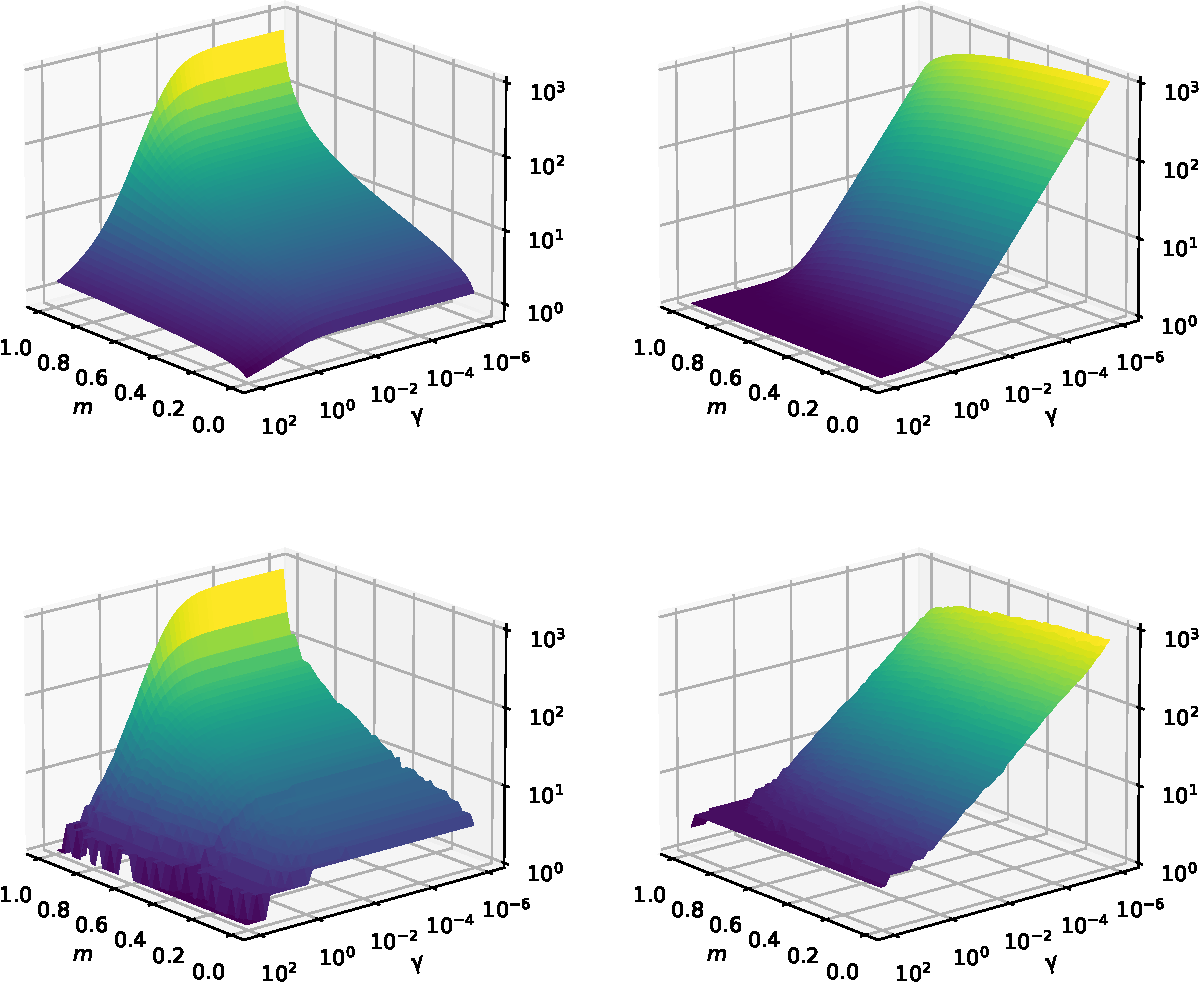
\includegraphics[width=\textwidth, angle=-1]{m_gamma_3d_plot_mpl}
};


\draw (-3.1,5.7) node {SIM};
\draw (3.3,5.7) node  {CGM};

\draw (-7,3) node  {Theoretical};
\draw (-7, -2.5) node  {Empirical};


% \draw (6.8,2.7) node {CGM};

% \draw (-4.2,0.3) node {$m=0.05$};
% \draw (-4.2,-4.7) node {$m=0.5$};
% \draw (-4.2,-9.7) node {$m=0.95$};


\end{tikzpicture}
\end{document} 
